\pagenumbering{Roman}
\chapter{Appendices}

\section{Project Schedule}
\begin{figure}[H]
	\centering
	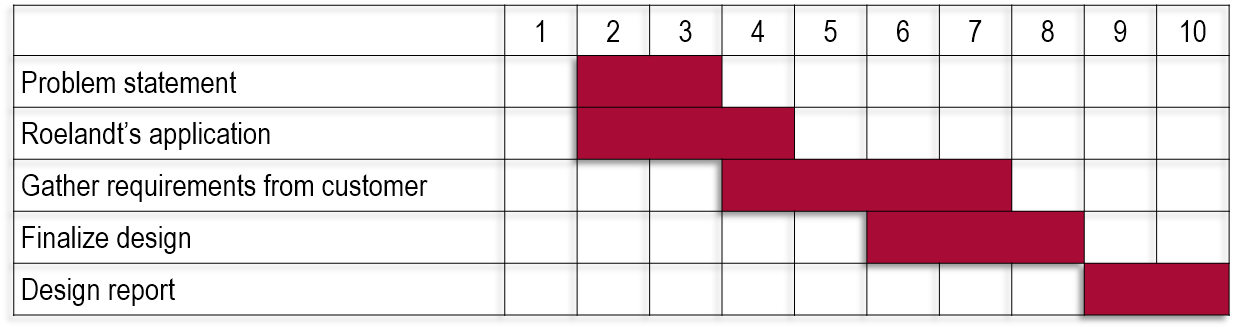
\includegraphics[scale=0.7]{schedule_fall.png}
	\caption{Gantt Chart for Fall Quarter}
\end{figure}

\begin{figure}[H]
	\centering
	
\includegraphics[scale=0.7]{schedule_winter.png}
	\caption{Gantt Chart for Winter Quarter}
\end{figure}

\begin{figure}[H]
	\centering
	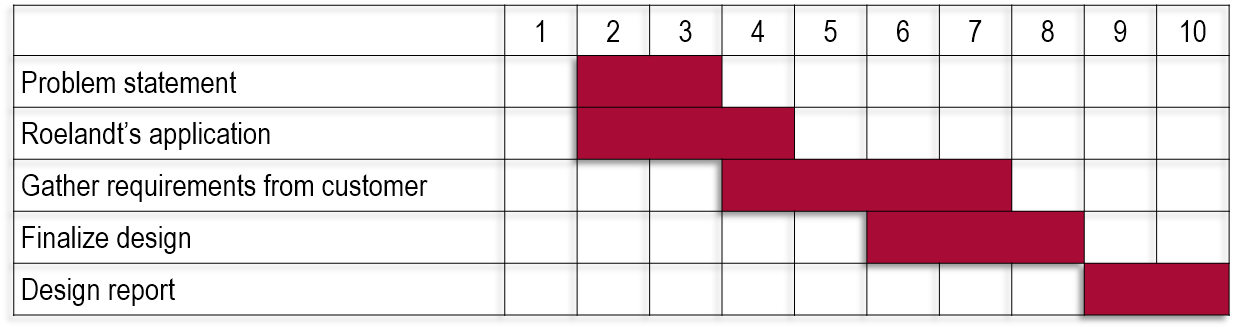
\includegraphics[scale=0.7]{schedule_fall.png}
	\caption{Gantt Chart for Spring Quarter}
\end{figure}

\begin{table}[H]
	\centering
	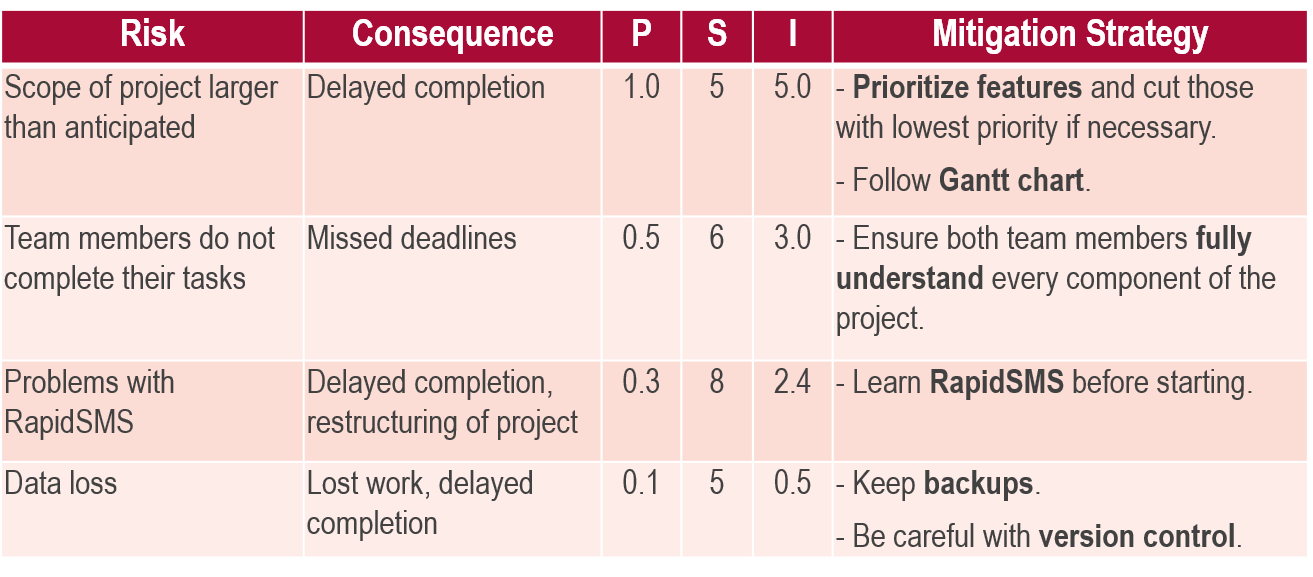
\includegraphics[scale=0.7]{risks.png}
	\caption{Risk Analysis}
\end{table}


\section{Setup and Installation}
This project is currently configured to be hosted on dotCloud with a Python server and PostgreSQL database and connects to a Tropo SMS backend. This manual will detail how to switch to your own subscription of dotCloud and Tropo and what to delete if you wish to replace Tropo with your own service.

\subsection*{General}
You will need Python on your system, Python 2.7 is recommended. https://www.python.org/download/releases/2.7
You will also ideally be using something unix based (Mac or Linux) if you are on a Windows machine try using Cygwin, but this has had mixed results.

\subsection*{Using your own dotCloud Credentials}
In order to deploy to dotCloud you will need to have python already installed on your computer. The code for this project was gotten from this github project, please see their documentation if you need additional instructions: https://github.com/caktus/rapidsms-deploy-dotcloud

Once you have Python 2.7 installed navigate to that folder through the terminal (or Cygwin) and follow the instructions in dotCloud installation instructions. http://docs.dotcloud.com/firststeps/install/
This will ask for your personal credentials, no changes to the code should be necessary.

You should now be able to push using “dotcloud push” in the terminal. This process may take some time

For adding custom domains see the following dotCloud documentation: http://docs.dotcloud.com/guides/domains/

\subsection*{Using your own Tropo backend}
You will need to modify code. You will need to get your account authorized before you can send outgoing messages. For help setting up your Tropo account  or trouble shooting the installation see this rapidSMS tutorial: http://rapidsms.readthedocs.org/en/latest/tutorial/tutorial04.html\#tutorial04

To complete this next part have your outgoing messaging token and Tropo phone number ready. 

\begin{enumerate}
	\item In the rapidsms\_tut folder open the settings.py file
	\item At nearly the bottom of the file, look for "INSTALLED\_BACKENDS = " in this section you should find 
	\begin{verbatim}
	    "my-tropo-backend": {
	        "ENGINE": "rtropo.outgoing.TropoBackend",
	        'config': {
	            'messaging\_token': '[insert_token]',
	            'number': '[+1-555-555-5555']’,
	        },
	    },
	\end{verbatim}
	\item Change the string under ‘messaging token’ to your messaging token
	\item Change the ‘number’ to you number, make sure you start with a ‘+’ followed by your country code
\end{enumerate}

\subsection*{Removing Tropo}
WARNING: Following these steps after you have created contacts with “my-tropo-backend” may result in critical errors. Be sure to delete any contacts with this backend first.

You will need to edit three files rapidsms\_tut/settings.py, rapidsms\_tut/urls.py, and requirements/base.py.

settings.py
\begin{enumerate}
	\item As in the previous section open settings.py in the rapidsms\_tut folder
	\item Delete the lines of code show in step 2 of the previous section

\subsubsection*{urls.py}
 	\item Open urls.py (also in the rapidsms\_tut folder)
	\item Delete the following lines of code:
    url(r'\^tropo/',
      message\_received,
      kwargs={'backend\_name': 'my-tropo-backend'}),
\subsubsection*{base.py}
	\item From the main folder navigate to the ‘requirements’ folder and open base.txt
	\item Delete the line rapidsms-tropo>=0.2.0

	\item After saving all these files, you should be able to “dotcloud push” and “my-tropo-backend” will no longer be available.
\end{enumerate}



\section{User Manual}

\section{Source Code}